\section{Project Results}
\label{sec:project_results}
The following section analyses the results obtained from the hardware and software developed in this project. The candidate successfully executes the minimal Linux OS in real hardware using the developed System on a chip. All the results obtained in this thesis which communicate with the FPGA board or the SoC testbench, are executing the developed \textit{Console} program. The hardware components comprising the SoC differ depending on the software needs.

\subsection{System Running "Hello World!"}

Table \ref{tab:hello_sim} shows a timing comparison between the different logic simulators simulating the \textbf{"Hello World!"} program in \textit{IOb-SoC-Linux}. The "INIT\_MEM" flag indicates whether the firmware is already loaded in the FPGA or if the \textit{Console} needs to transfer the firmware to the SoC, the user can set the flag to '1' or '0' respectively. The users can execute the simulations with or without external memory. Furthermore, the firmware can run in internal or external memory. The "make sim-test" command tests the different possible simulations.

\begin{table}[!ht]
    \centering
    \begin{tabular}{l|ll|}
    \cline{2-3}
                                          & \multicolumn{1}{l|}{\textbf{Icarus}}  & \textbf{Verilator} \\ \hline
    \multicolumn{1}{|l|}{INIT\_MEM=1}     & \multicolumn{1}{l|}{2m 26s}           & 0m 3s              \\ \hline
    \multicolumn{1}{|l|}{INIT\_MEM=0}     & \multicolumn{1}{l|}{88m 19s}          & 1m 1s              \\ \hline
    \multicolumn{1}{|l|}{all simulations} & \multicolumn{1}{l|}{231m 3s}          & 2m 27s             \\ \hline
    \end{tabular}
    \caption{Timing the "Hello World!" firmware simulation.}
    \label{tab:hello_sim}
\end{table}

From table \ref{tab:hello_sim} engineers are able to conclude the advantage of using \textit{Verilator}. For more complexed systems the \textit{C++} testbench is much faster than the \textit{Verilog} counterpart. The disadvantage of using \textit{Verilator} is that signal values can only be either '0' or '1'. However, the speed-up in the simulation is also due to the signal value limitation. In \textit{Icarus}, the simulation can evaluate the signal as unknown ('x') when they are uninitialised. The author noted that \textit{Verilator} is slower to compile the testbench. However, it is much faster to execute the software.

In figure \ref{fig:hello_fpga} the readers can see the output of executing the "Hello World!" firmware in the FPGA. The author synthesised the SoC with the external memory. Furthermore, the firmware is running from external memory.

\begin{figure}[!ht]
    \centering
    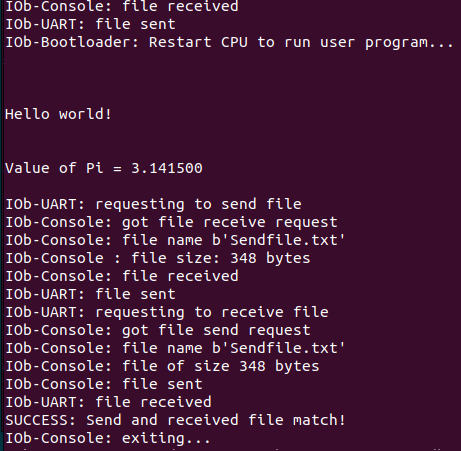
\includegraphics[width=\linewidth]{../images/end_hello_fpga.png}
    \caption{Running the "Hello World!" firmware in the FPGA Board.}
    \label{fig:hello_fpga}
\end{figure}

Tables \ref{tab:cyclone_hello} and \ref{tab:kintex_hello} are the FPGA implementation results for two FPGA families. The author implemented the developed SoC on the kintex Ultrascale AES-KU040-DB-G board and in the CYCLONE V GT-DK. \textit{IOb-SoC-Linux} implemented in this section only contains the swapped CPU. Furthermore, \textit{IOb-SoC-Linux} uses the external memory to run the firmware from there.

\begin{table}[!ht]
    \centering
    \begin{tabular}{l|l|l|}
        \cline{2-3}
                                          & \textit{IOb-SoC-Linux} & \textit{IOb-SoC} \\ \hline
        \multicolumn{1}{|l|}{ALM}         & 10,062                 & 9,280            \\ \hline
        \multicolumn{1}{|l|}{FF}          & 12150                  & 10020            \\ \hline
        \multicolumn{1}{|l|}{DSP}         & 8                      & 3                \\ \hline
        \multicolumn{1}{|l|}{BRAM blocks} & 234                    & 352              \\ \hline
        \multicolumn{1}{|l|}{BRAM bits}   & 753,248                & 779,744          \\ \hline
    \end{tabular}
    \caption{Cyclone V GT}
    \label{tab:cyclone_hello}
\end{table}
\begin{table}[!ht]
    \centering
    \begin{tabular}{l|l|l|}
        \cline{2-3}
                                        & \textit{IOb-SoC-Linux} & \textit{IOb-SoC} \\ \hline
        \multicolumn{1}{|l|}{LUTs}      & 21226                  & 23003            \\ \hline
        \multicolumn{1}{|l|}{Registers} & 23373                  & 22588            \\ \hline
        \multicolumn{1}{|l|}{DSPs}      & 10                     & 7                \\ \hline
        \multicolumn{1}{|l|}{BRAM}      & 39.5                   & 34.5             \\ \hline
        \multicolumn{1}{|l|}{BRAM bits} & 1422000                & 1242000          \\ \hline
    \end{tabular}
    \caption{Kintex Ultrascale}
    \label{tab:kintex_hello}
\end{table}

\subsection{Interrupt Routines}
After developing the \textbf{CLINT} unit, the author executed its testbench, testing the timer and software interrupts. Figure~\ref{fig:clint_sim} shows the complete process when running a simulation.

\begin{figure}[!ht]
    \centering
    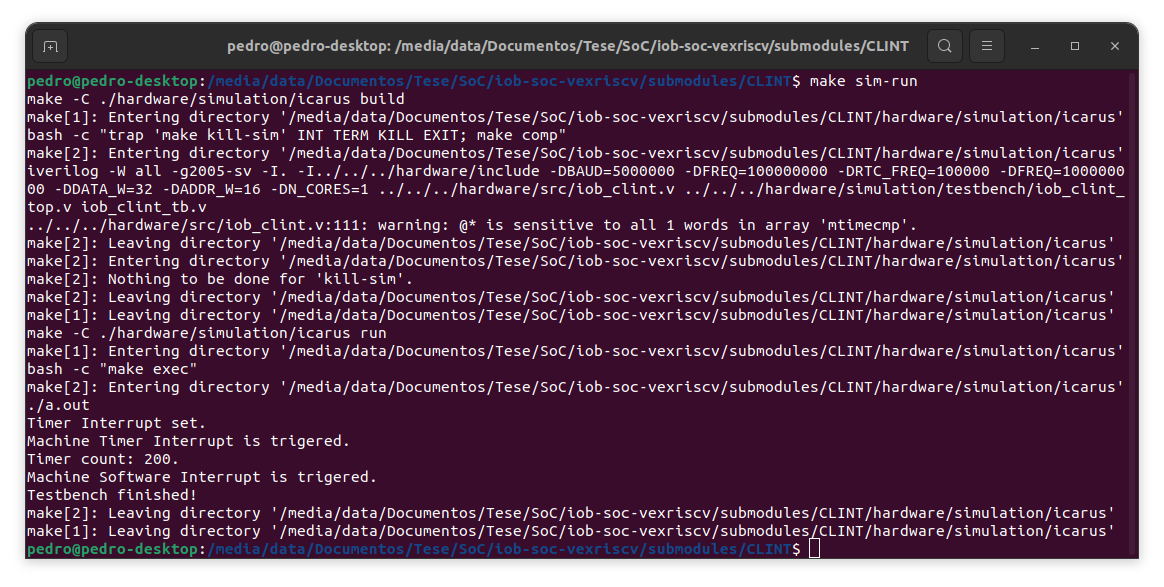
\includegraphics[width=\linewidth]{../images/clint_sim.png}
    \caption{CLINT timer and software interrupt simulation.}
    \label{fig:clint_sim}
\end{figure}

Figure \ref{fig:int_sim} shows the execution of the \textbf{interrupt routine firmware}. The \textit{IOb-SoC-Linux} implemented in simulation does not use external memory.

\begin{figure}[!ht]
    \centering
    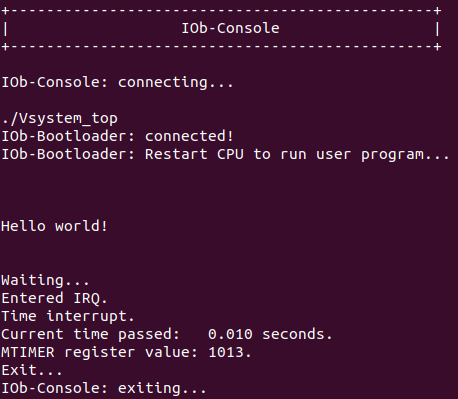
\includegraphics[width=\linewidth]{../images/verilator_int_sim.png}
    \caption{Running the interrupt routine firmware in simulation.}
    \label{fig:int_sim}
\end{figure}

Figure~\ref{fig:int_fpga} shows the execution of the firmware from the \textit{IOb-SoC-Linux} internal memory in the \textbf{FPGA}. The firmware programs the timer interrupt to trigger one second after the firmware starts. The interrupt handler prints the current time that has passed since the firmware started. The hardware waited one second for the interrupt to trigger. The extra 0.004 seconds are to print the "Hello World" message at the start of the firmware and to execute the interrupt handler. The extra time consumed when executing the \textit{IOb-SoC-Linux} in hardware differs from the simulation's extra time due to the baud rate used. Since the hardware baud rate is lower than the simulation baud rate, the messages theoretically take more time to print to the terminal.

\begin{figure}[!ht]
    \centering
    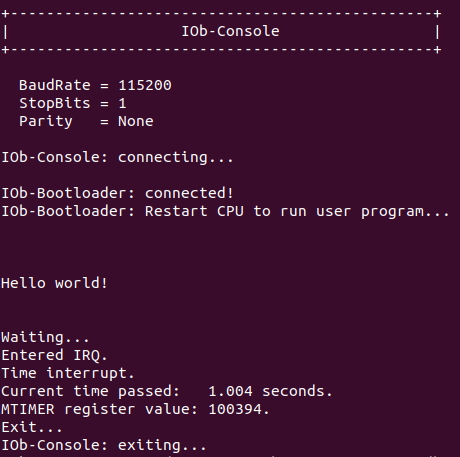
\includegraphics[width=\linewidth]{../images/int_fpga.png}
    \caption{Executing the interrupt routine program on the FPGA.}
    \label{fig:int_fpga}
\end{figure}

Tables \ref{tab:cyclone_int} and \ref{tab:kintex_int} represent how much FPGA resources are consumed by the \textit{IOb-SoC-Linux}. The author executed the firmware from the external memory and the internal memory.

\begin{table}[!ht]
    \centering
    \begin{tabular}{|l|l|}
        \hline
        ALM         & 10,257  \\ \hline
        FF          & 12300   \\ \hline
        DSP         & 8       \\ \hline
        BRAM blocks & 234     \\ \hline
        BRAM bits   & 753,248 \\ \hline
    \end{tabular}
    \caption{Cyclone V GT}
    \label{tab:cyclone_int}
\end{table}
\begin{table}[!ht]
    \centering
    \begin{tabular}{|l|l|l|}
        \hline
        LUTs      & 21478   \\ \hline
        Registers & 23545   \\ \hline
        DSPs      & 10      \\ \hline
        BRAM      & 39.5    \\ \hline
        BRAM bits & 1422000 \\ \hline
    \end{tabular}
    \caption{Kintex Ultrascale}
    \label{tab:kintex_int}
\end{table}

Comparing table \ref{tab:kintex_int} and~\ref{tab:cyclone_int} with the table \ref{tab:kintex_hello} engineers can see that the CLINT hardware does not use much resources.

\subsection{Boot and use the Linux Operating System}

The objective of this thesis project was to run an Operating System in the \textit{IOb-SoC-Linux}. Table \ref{tab:time_os} presents how much time it takes to build the complete OS with the command "make build-OS". The "real" time is the time that passes since the user executes the command until it finishes. The "user" time is the time the CPU takes while executing operations in the user space. The "user" time is bigger than the "real" time because it counts the time passed in each CPU core. Part of the compilation of the RootFS and the kernel is done in parallel using two cores.

\begin{table}[!ht]
    \centering
    \begin{tabular}{ll}
    real & 4m29,570s \\
    user & 8m12,039s \\
    sys  & 0m56,887s
    \end{tabular}
    \caption{Time it takes to build the OS.}
    \label{tab:time_os}
\end{table}

The OS size is to big to run in the FPGA internal memory. Consequently, the author had to implement the \textit{IOb-SoC-Linux} on the FPGA with access to the external memory. Figures \ref{fig:start_bootloader_sim} and \ref{fig:end_bootloader_sim} show the start of the OS simulation with \textit{Verilator}.

\begin{figure}[!ht]
    \centering
    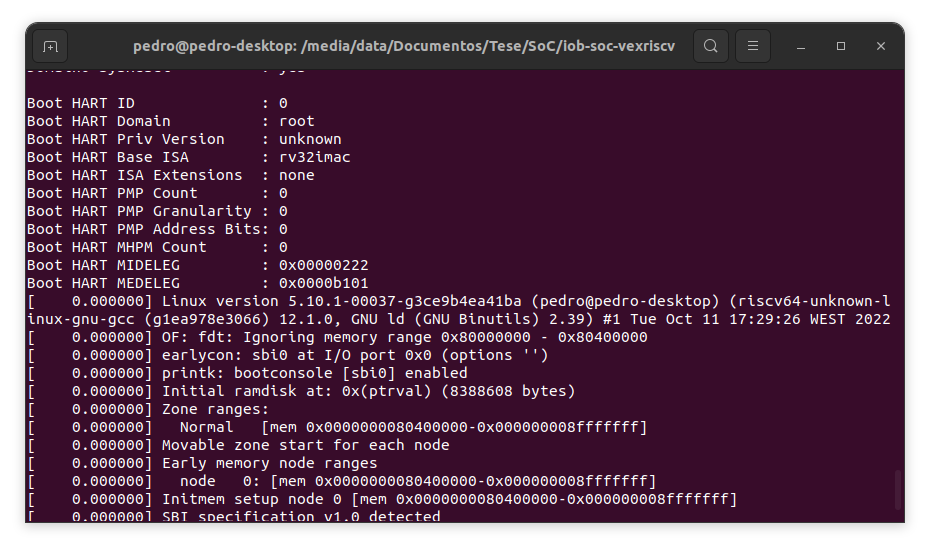
\includegraphics[width=\linewidth]{../images/start_Linux_sim.png}
    \caption{\textit{iob-UART16550} and \textit{iob-PLIC} properties.}
    \label{fig:start_bootloader_sim}
\end{figure}
\begin{figure}[!ht]
    \centering
    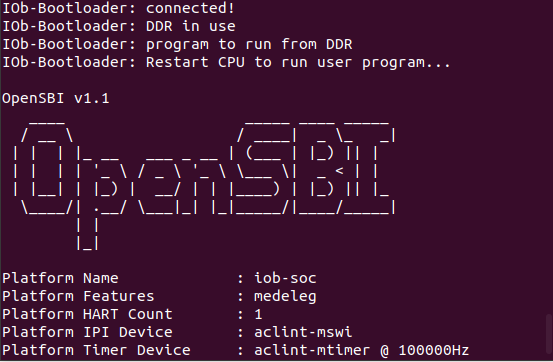
\includegraphics[width=\linewidth]{../images/end_bootloader_sim.png}
    \caption{\textit{IOb-SoC} bootloader and \textit{OpenSBI} firmware.}
    \label{fig:end_bootloader_sim}
\end{figure}

Figure \ref{fig:start_bootloader_sim} shows the initialization of the \textit{Console} program. Furthermore, it shows the instantiation of the \textit{iob-UART16550} and the \textit{iob-PLIC}. The \textit{iob-UART16550} and the PLIC core have an initial block that prints their properties. The synthesis tools do not synthesise the initial block to real hardware, but the simulator executes it. Figure \ref{fig:end_bootloader_sim} shows the \textit{iob-bootloader} and the start of the \textit{OpenSBI} bootloader. Figure \ref{fig:start_linux_sim} shows the end of the \textit{OpenSBI} bootloader and the start of the Linux kernel. The first line printed by the Linux kernel indicates the author built the kernel executing, the kernel version and which toolchain he used to compile it.

\begin{figure}[!ht]
    \centering
    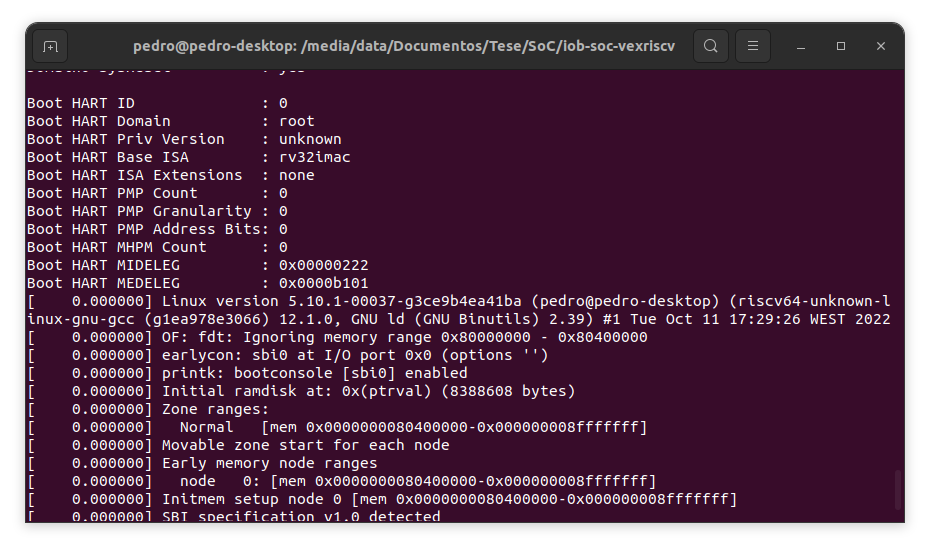
\includegraphics[width=\linewidth]{../images/start_Linux_sim.png}
    \caption{Start of the Linux kernel boot with \textit{Verilator}.}
    \label{fig:start_linux_sim}
\end{figure}

While figure \ref{fig:start_linux_sim} shows the start of the Linux kernel, figure \ref{fig:end_linux_verilator} shows the end of the Linux kernel booting process and the execution of the "init" script. The "init" script is the first program the OS executes after the Linux kernel mounts the RootFS and finishes booting. There exist multiple messages printed to the terminal between the output shown in figure \ref{fig:start_linux_sim} and in \ref{fig:end_linux_verilator}. Those messages show the progress while the Linux kernel boots. The Linux kernel boot process's last message is "Run /init as init process". After that message the SoC executes the "init" program.

\begin{figure}[!ht]
    \centering
    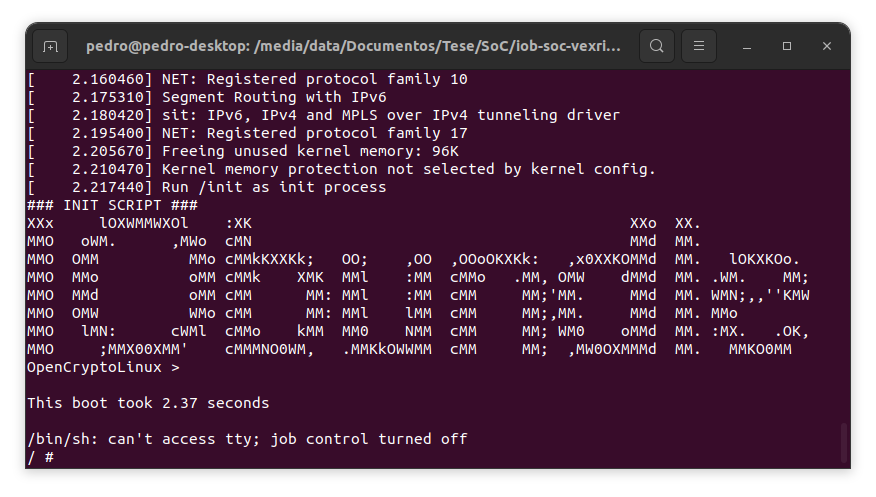
\includegraphics[width=\linewidth]{../images/end_Linux_sim.png}
    \caption{End of Linux kernel boot with \textit{Verilator}.}
    \label{fig:end_linux_verilator}
\end{figure}

Figure \ref{fig:linux_fpga} shows the developed minimal OS running on an FPGA. The reader can see that the author has suppressed the shell warning. The initial part of the figure shows the final stage of the Linux kernel booting. After booting, the author tested the \textit{"ls /"} command that showed the files and directories in the systems' root. Lastly the author executed the \textit{"cat init"} command for the OS to print the contents of the "init" script to the terminal.

\begin{figure}[!ht]
    \centering
    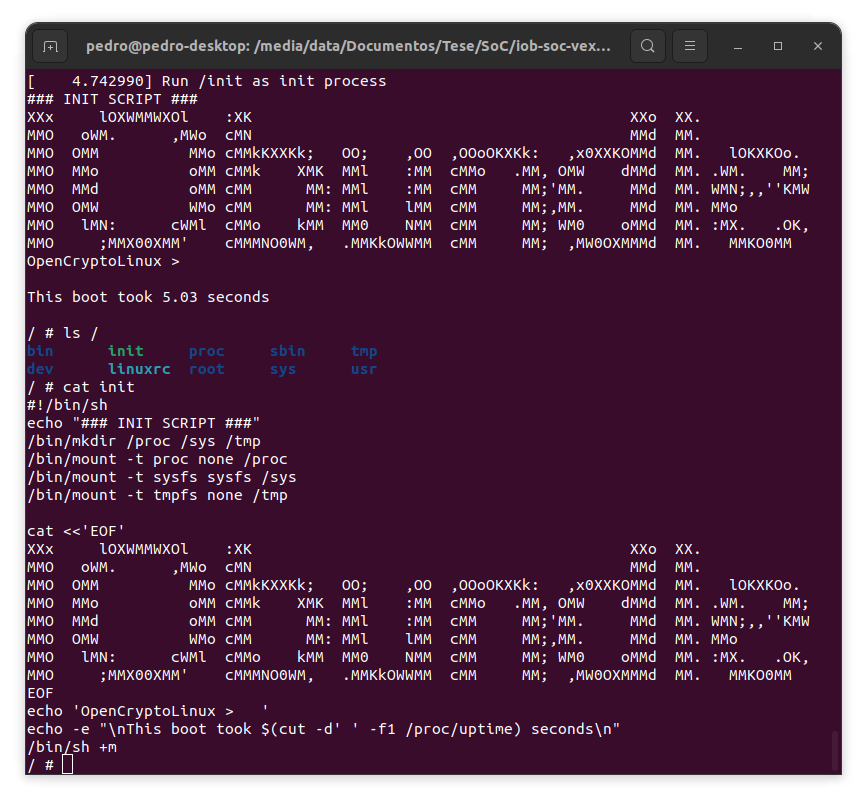
\includegraphics[width=\linewidth]{../images/linux_fpga.png}
    \caption{Linux kernel boot in the FPGA.}
    \label{fig:linux_fpga}
\end{figure}

The time the Linux kernel takes to boot in real hardware, figure \ref{fig:linux_fpga}, is almost double what it takes to boot in simulation, figure \ref{fig:linux_fpga}. The time to boot is almost double because the memory module used in the simulation does not have any latency. When the L2 cache fetches data from memory in real hardware, it must wait before receiving the data burst. Using the \textit{CYCLONE V} FPGA board the Linux kernel takes 7.01 seconds to boot. The \textit{Kintex Ultrascale} runs with a frequency of 100 MHz, and the \textit{CYCLONE V} runs at 50 MHz. The \textit{OpenSBI} bootloader and the device tree blob had to be recompiled with the system frequency defined to 50 MHz to run in the \textit{CYCLONE V}.

A more complex rootfs generated with \textit{Buildroot} provides more features than the minimal rootfs developed. The \textit{Buildroot} rootfs allows using \textit{MicroPython}~\cite{tollervey2017programming} in \textit{IOb-SoC-Linux} and executing the \textit{Dhrystones}~\cite{weicker1984dhrystone} benchmarking software. Figure \ref{fig:linux_buildroot_fpga} shows the final output of the \textit{Dhrystones} benchmark and the execution of simple commands in \textit{MicroPython}.

\begin{figure}[!ht]
    \centering
    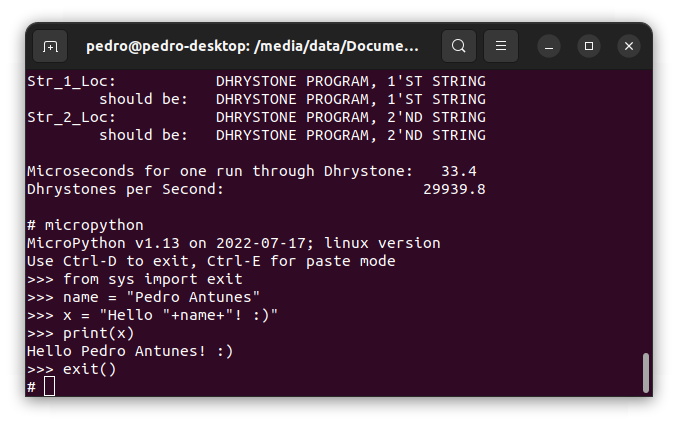
\includegraphics[width=\linewidth]{../images/linux_buildroot_fpga.png}
    \caption{Linux OS with \textit{Buildroot} rootfs.}
    \label{fig:linux_buildroot_fpga}
\end{figure}

\textit{MicroPython} is a software project that aims to implement a \textit{Python} version, highly compatible with \textit{Python3}, in microcontrollers and small embedded systems. \textit{Dhrystones} is a general-performance benchmarking software used in multiple embedded systems. A common representation of the \textit{Dhrystones} benchmark is \textit{DMIPS}. Table \ref{tab:dhrystones} represents a comparison between the \textit{Dhrystones} benchmarking scores of both FPGA boards.

\begin{table}[!ht]
    \centering
    \begin{tabular}{l|l|l|}
    \cline{2-3}
                                & \textbf{Kintex Ultrascale} & \textbf{CYCLONE V} \\ \hline
    \multicolumn{1}{|l|}{DMIPS} & 23.33                      & 17.04              \\ \hline
    \end{tabular}
    \caption{\textit{Dhrystones} benchmarking.}
    \label{tab:dhrystones}
\end{table}

Tables \ref{tab:kintex_linux} and \ref{tab:cyclone_linux} show the resources used by the \textit{IOb-SoC-Linux} in the different FPGAs.

\begin{table}[!ht]
    \centering
    \begin{tabular}{l|l|l|}
        \cline{2-3}
                                            & Resources & FPGA usage \% \\ \hline
        \multicolumn{1}{|l|}{ALM}         & 11,227    & 10                       \\ \hline
        \multicolumn{1}{|l|}{DSP}         & 8         & 3                        \\ \hline
        \multicolumn{1}{|l|}{FF}          & 13725     & 2                        \\ \hline
        \multicolumn{1}{|l|}{BRAM blocks} & 234       & 19                       \\ \hline
        \multicolumn{1}{|l|}{BRAM bits}   & 755,424   & 9                        \\ \hline
    \end{tabular}
    \caption{Cyclone V GT}
    \label{tab:cyclone_linux}
\end{table}
\begin{table}[!ht]
    \centering
    \begin{tabular}{l|l|l|}
        \cline{2-3}
                                        & Resources & FPGA usage \% \\ \hline
        \multicolumn{1}{|l|}{LUTs}      & 23126     & 9.54                     \\ \hline
        \multicolumn{1}{|l|}{Registers} & 24505     & 5.05                     \\ \hline
        \multicolumn{1}{|l|}{DSPs}      & 10        & 0.52                     \\ \hline
        \multicolumn{1}{|l|}{BRAM}      & 39.5      & 6.58                     \\ \hline
    \end{tabular}
    \caption{Kintex Ultrascale}
    \label{tab:kintex_linux}
\end{table}

Tables in \ref{tab:kintex_linux} and \ref{tab:cyclone_linux} show that the resources utilization from the \textit{IOb-SoC-Linux} is less than 10\% in the supported FPGA boards. Comparing the tables \ref{tab:kintex_linux} and \ref{tab:cyclone_linux} with the tables in \ref{tab:kintex_hello} and \ref{tab:cyclone_hello} it is clear the \textit{IOb-SoC-Linux} does not use many more resources than the \textit{IOb-SoC}.